% Created 2016-08-06 Sat 23:31

\documentclass[nofonts]{ctexart}
\author{Robin}
\setCJKmainfont[ItalicFont={AR PL UKai CN}]{AR PL UMing CN} 
\setCJKsansfont{WenQuanYi Zen Hei} 
\setCJKmonofont{WenQuanYi Zen Hei Mono} 

\usepackage{hyperref}
\usepackage[utf8]{inputenc}
\usepackage{fixltx2e}
\usepackage{graphicx}
\usepackage{longtable}
\usepackage{float}
\usepackage{wrapfig}
\usepackage{rotating}
\usepackage[normalem]{ulem}
\usepackage{amsmath}
\usepackage{textcomp}
\usepackage{marvosym}
\usepackage{wasysym}
\usepackage{multicol}
\usepackage{amssymb}
\tolerance=1000
\date{\today}
\title{My little document}
\hypersetup{
 pdfauthor={},
 pdftitle={My little document},
 pdfkeywords={},
 pdfsubject={},
 pdfcreator={Emacs 24.5.1 (Org mode 8.3.5)}, 
 pdflang={English}}
\begin{document}

\maketitle
\tableofcontents

\section{latex测试}
\label{sec:orgheadline10}
\subsection{公式}
\label{sec:orgheadline1}
\(\frac{1}{\sqrt{2\pi\sigma^2}}e^{ -\frac{(x-\mu)^2}{2\sigma^2} }\)
\subsection{表格caption}
\label{sec:orgheadline2}
    表格的问题是,caption显示的位置在顶部,
    而且表格并不居中,本来想测试下pdf的效果,不过latex坏了.所以暂且放着
应该是可以解决的问题吧.
$\backslash$#+ATTR\(_{\text{HTML}}\): class="center"

\begin{table}[htb]
\caption{\label{tab:orgtable1}
This is the caption for the next table (or link)}
\centering
\begin{tabular}{llll}
awef & aiwfeofj & afaw & safwea\\
\hline
afiwoefj & fwiaoejfi & fjiweoaf & fe\\
sfajwief & s &  & \\
 &  &  & \\
\end{tabular}
\end{table}

\subsection{?}
\label{sec:orgheadline3}
\subsection{图片caption}
\label{sec:orgheadline4}

\begin{figure}[htb]
\centering
\includegraphics[width=.9\linewidth]{img/1.jpg}
\caption{\label{fig:orgparagraph1}
This is the caption for the next figure link (or table)}
\end{figure}

emacs中的文件补全还不熟悉,所以文件路径编辑可能要用vim做.
\subsection{1.jpg}
\label{sec:orgheadline5}
\begin{figure}[htb]
\centering
\includegraphics[width=.9\linewidth]{1.jpg}
\caption{\label{fig:orgparagraph2}
1.jpg}
\end{figure}
\subsection{img/1.jpg}
\label{sec:orgheadline6}
\begin{figure}[htb]
\centering
\includegraphics[width=.9\linewidth]{img/1.jpg}
\caption{\label{fig:orgparagraph3}
img/1.jpg}
\end{figure}
\subsection{?}
\label{sec:orgheadline7}
./images/screenshot/depth.png
./images/screenshot/stereo\(_{\text{1channel.png}}\)
\subsection{问题}
\label{sec:orgheadline8}
之前这份文件转换到latex pdf是没有问题的,但是似乎这天电脑上的什么配置被搞坏了,
所以只有等到之后有时间重装下系统来修复了,所以暂时只能输出html了
\subsection{pdf测试结果}
\label{sec:orgheadline9}
虽然xelatex在转换中报错了,但是结果很好
表格是居中的,不过caption在顶部
图片显示正常

字体有缺失,标题中的中文显示不了
\end{document}
